% !TeX root = p2p.tex

\section*{Appendix B: project code overview}

Simulations are based on the \emph{cycle-driven} engine of \peersim{}. This seems a natural choice given the synchronous communication model assumption, but the way in which the engine handles the execution of the protocol code required some adjustments. When dealing with cycle-driven protocols, \peersim{} executes each simulation cycle sequentially by iterating through the \texttt{Node} instances that form the network and invoking the \texttt{nextCycle} method that the protocol implements. If precautions are not taken, this execution policy clashes with the synchronous model assumption: if a node $n$ has two neighbors that at the current step need to interact with it (for example to communicate the number of shortest paths) and one of them is executed after $n$ in the iteration order, the information will be available to $n$ only at the following cycle.

Rather than adapting the protocol code to be mindful of this potential situation, the choice was to include the synchronous communication model in the simulation. A synchronous protocol is a \texttt{CDProtocol} that can send messages to other synchronous protocols with the guarantee that those will be received after the \texttt{nextCycle} method will be invoked by the simulator on the receiver at the current step, but before the invocation at the following step. This allows to execute each simulation cycle at each node in isolation, only using information generated in the previous cycle exactly as the synchronous communication model assumption requires. This is achieved by implementing the \texttt{CycleBasedTransportSupport} interface:
\begin{minted}{text}
public interface CycleBasedTransportSupport<T> {
    interface SendQueueEntry<T> {
        T getMessage();
        CycleBasedTransportSupport<T> getDestination();
    }
    void addToSendQueue(T message, CycleBasedTransportSupport<T> destination);
    boolean hasOutgoingMessages();
    void addToIncoming(T message);
    Iterator<T> getIncomingMessagesIterator();
    Iterator<SendQueueEntry<T>> getSendQueueIterator();
}
\end{minted}
This generic interface offers facilities to synchronously transfer objects between protocols that implement it. The \texttt{addToSendQueue} method should temporarily store the message and the destination in a send queue, which is then iterated by a \texttt{CycleBasedTransport} control at the end of a cycle in order to deliver each message to the appropriate destination. A protocol can then call the \texttt{getIncomingMessageIterator} method in the next cycle and iterate through the received messages.

\subsection*{Messages}
The messages exchanged by the protocols during the simulation are instances of the \texttt{Message} class. This class provides factory methods to generate \mdisc{} and \mrep{} message objects that follow the conventions used in the definition of the algorithms. 

\subsection*{Protocol classes}

\begin{figure}
\centering
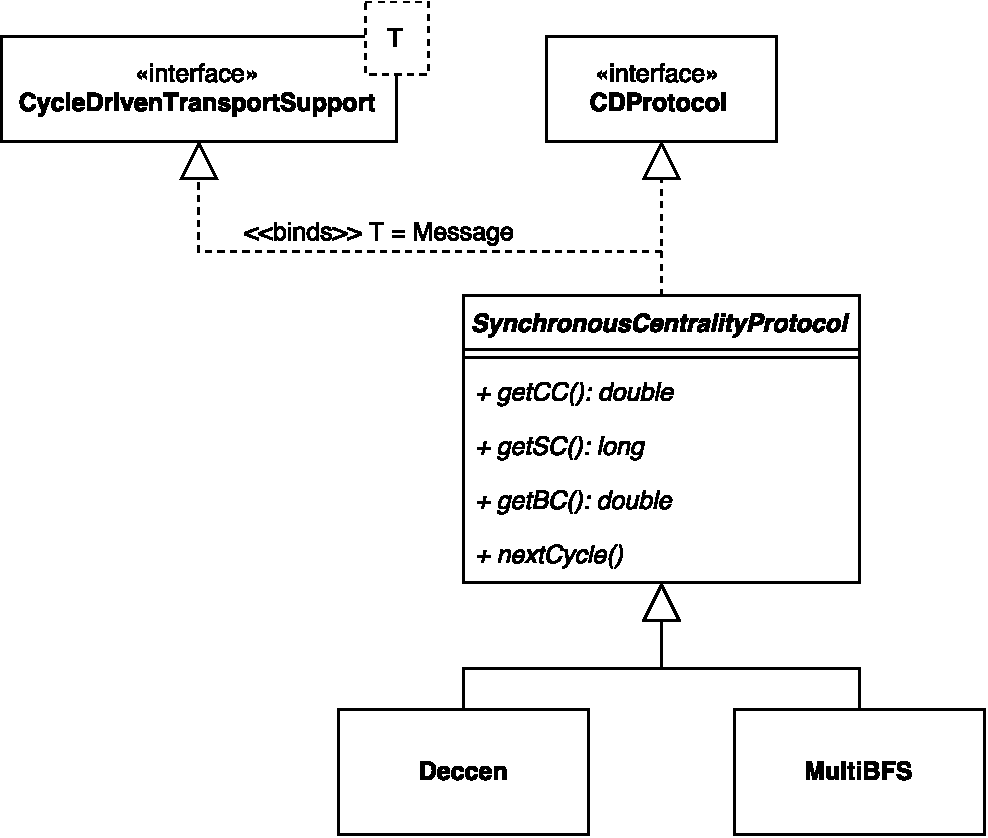
\includegraphics[width=0.72\textwidth]{diagram.pdf}
\caption{Class diagram [TODO]}
\label{class:protocol:hierarchy}
\end{figure}

Protocol classes are organized in the hierarchy shown in figure \ref{class:protocol:hierarchy}. The abstract class \texttt{SynchronousCentralityProtocol} implements the \texttt{Cycle\allowbreak Based\-Transport\-Support<Message>}  interface, while the \texttt{nextCycle()} method of the PeerSim interface \texttt{CDProtocol} is declared \texttt{abstract}.

The implementation of the protocols is straightforward and very similar to the descriptions given previously.

\subsection*{\deccen{} protocol implementation}

The \texttt{Deccen} class implements a \deccen{} node in the simulator. A node needs to keep track of the shortest path information it has collected and of the reports it has handled.
\begin{minted}{text}
public class Deccen extends SynchronousCentralityProtocol {
    private static class ShortestPathData {
        public final int count;
        public final int length;

        public ShortestPathData(int count, int length) {
            this.count = count;
            this.length = length;
        }
    }

    private static class OrderedPair<T1,T2> {
        public final T1 first;
        public final T2 second;

        public OrderedPair(T1 first, T2 second) {
            this.first = first;
            this.second = second;
        }
        ...
    }
    ...
    private Map<Node, ShortestPathData> shortestPathMap;
    private Set<OrderedPair<Long,Long>> handledReports;
    ...
}
\end{minted}
Listing \ref{listing:deccen} reports an excerpt of the \texttt{Deccen} class. The \texttt{shortestPathMap} map is used to store relevant information about the shortest paths to other nodes and is updated whenever new \mdisc{} messages are received while reports are tracked with \texttt{handledReports} set of \texttt{Node} ID pairs.

The \texttt{nextCycle()} method simply executes the actions described in section \ref{deccen:step}:
\begin{minted}{java}
public void nextCycle(Node self, int protocolID) {
    Map<Node,List<Message>> discoveryMap = new HashMap<Node,List<Message>>();
    List<Message> reportList = new LinkedList<Message>();
    parseIncomingMessages(discoveryMap, reportList);
    if (!discoveryMap.isEmpty()) processDiscoveryMessages(self, protocolID, discoveryMap);
    if (!reportList.isEmpty()) processReportMessages(self, protocolID, reportList);
}
\end{minted}

\subsection*{\multibfs{} protocol implementation}

The state of a \multibfs{} node mainly consists of a dictionary to keep track of the various visits that are performed during the algorithm execution.

\begin{minted}{text}
public class MultiBFS extends SynchronousCentralityProtocol {
    private static class VisitState {
        ...
    }
    ...
    private Map<Node, VisitState> activeVisits;
    private Set<Node> completed;
    ...
    public boolean isWaiting(Node source) { ... }
    public boolean isActive(Node source) { ... }
    public boolean isCompleted(Node source) { ... }
}
\end{minted}
Recall that the state of a node is parametric with respect to each source of a visit. The state is \swait{\texttt{s}} if the \texttt{Node} instance \texttt{s} does not appear as key in the \texttt{activeVisits} map and neither is contained in the \texttt{completed} set; this is the initial state for any source since both structures are empty at the start of the protocol. When a node is in state \sact{\texttt{s}} an entry with key \texttt{s} is present in the \texttt{activeVisits} map. After a node has reported back to all the predecessors, it changes state \scomp{\texttt{s}} by removing the mapping from \texttt{activeVisits} and inserting \texttt{s} in the \texttt{completed} set.

Entries in the \texttt{activeVisits} map are used to store data while a node is in the ``active'' phase. A \texttt{VisitState} object is used to keep track of the predecessors and children sets, and to incrementally compute the values to be reported to the predecessor nodes:
\begin{minted}{text}
private static class VisitState {
    public Set<Node> predecessors;
    public Set<Node> siblings;
    public Set<Node> children;
    public int distanceFromSource;
    public int timestamp;
    public int sigma;
    public long contributionSC;
    public double contributionBC;
    ...	
    public void accumulate(Node child, double bcc, long scc, int numSP) {
        ...
    }
}
\end{minted}
The \texttt{accumulate()} method updates the centrality contributions by applying the recursive relations \eqref{eq:th:contrib:bc} and \eqref{eq:th:contrib:sc}, and is invoked whenever a child node sends a report.

Finally, the implementation of the \texttt{nextCycle()} method which closely follows the specification given in section \ref{multibfs:step}:
\begin{minted}{text}
public void nextCycle(Node self, int protocolID) {
    Map<Node,List<Message>> discoveryMap = new HashMap<Node,List<Message>>();
    List<Message> reportList = new LinkedList<Message>();
    parseIncomingMessages(discoveryMap, reportList);
    if (!discoveryMap.isEmpty()) processDiscoveryMessages(self, protocolID, discoveryMap);
    if (!reportList.isEmpty()) processReportMessages(reportList);
    reportNewCompleted(self, protocolID);
}
\end{minted}
Messages are parsed and handled by type, then active visits for which all child nodes have reported are finalized with the \texttt{reportNewCompleted()} method by integrating the contributions in the centrality accumulators and reporting the relevant data to each predecessor.